\documentclass[1p]{elsarticle_modified}
%\bibliographystyle{elsarticle-num}

%\usepackage[colorlinks]{hyperref}
%\usepackage{abbrmath_seonhwa} %\Abb, \Ascr, \Acal ,\Abf, \Afrak
\usepackage{amsfonts}
\usepackage{amssymb}
\usepackage{amsmath}
\usepackage{amsthm}
\usepackage{scalefnt}
\usepackage{amsbsy}
\usepackage{kotex}
\usepackage{caption}
\usepackage{subfig}
\usepackage{color}
\usepackage{graphicx}
\usepackage{xcolor} %% white, black, red, green, blue, cyan, magenta, yellow
\usepackage{float}
\usepackage{setspace}
\usepackage{hyperref}

\usepackage{tikz}
\usetikzlibrary{arrows}

\usepackage{multirow}
\usepackage{array} % fixed length table
\usepackage{hhline}

%%%%%%%%%%%%%%%%%%%%%
\makeatletter
\renewcommand*\env@matrix[1][\arraystretch]{%
	\edef\arraystretch{#1}%
	\hskip -\arraycolsep
	\let\@ifnextchar\new@ifnextchar
	\array{*\c@MaxMatrixCols c}}
\makeatother %https://tex.stackexchange.com/questions/14071/how-can-i-increase-the-line-spacing-in-a-matrix
%%%%%%%%%%%%%%%

\usepackage[normalem]{ulem}

\newcommand{\msout}[1]{\ifmmode\text{\sout{\ensuremath{#1}}}\else\sout{#1}\fi}
%SOURCE: \msout is \stkout macro in https://tex.stackexchange.com/questions/20609/strikeout-in-math-mode

\newcommand{\cancel}[1]{
	\ifmmode
	{\color{red}\msout{#1}}
	\else
	{\color{red}\sout{#1}}
	\fi
}

\newcommand{\add}[1]{
	{\color{blue}\uwave{#1}}
}

\newcommand{\replace}[2]{
	\ifmmode
	{\color{red}\msout{#1}}{\color{blue}\uwave{#2}}
	\else
	{\color{red}\sout{#1}}{\color{blue}\uwave{#2}}
	\fi
}

\newcommand{\Sol}{\mathcal{S}} %segment
\newcommand{\D}{D} %diagram
\newcommand{\A}{\mathcal{A}} %arc


%%%%%%%%%%%%%%%%%%%%%%%%%%%%%5 test

\def\sl{\operatorname{\textup{SL}}(2,\Cbb)}
\def\psl{\operatorname{\textup{PSL}}(2,\Cbb)}
\def\quan{\mkern 1mu \triangleright \mkern 1mu}

\theoremstyle{definition}
\newtheorem{thm}{Theorem}[section]
\newtheorem{prop}[thm]{Proposition}
\newtheorem{lem}[thm]{Lemma}
\newtheorem{ques}[thm]{Question}
\newtheorem{cor}[thm]{Corollary}
\newtheorem{defn}[thm]{Definition}
\newtheorem{exam}[thm]{Example}
\newtheorem{rmk}[thm]{Remark}
\newtheorem{alg}[thm]{Algorithm}

\newcommand{\I}{\sqrt{-1}}
\begin{document}

%\begin{frontmatter}
%
%\title{Boundary parabolic representations of knots up to 8 crossings}
%
%%% Group authors per affiliation:
%\author{Yunhi Cho} 
%\address{Department of Mathematics, University of Seoul, Seoul, Korea}
%\ead{yhcho@uos.ac.kr}
%
%
%\author{Seonhwa Kim} %\fnref{s_kim}}
%\address{Center for Geometry and Physics, Institute for Basic Science, Pohang, 37673, Korea}
%\ead{ryeona17@ibs.re.kr}
%
%\author{Hyuk Kim}
%\address{Department of Mathematical Sciences, Seoul National University, Seoul 08826, Korea}
%\ead{hyukkim@snu.ac.kr}
%
%\author{Seokbeom Yoon}
%\address{Department of Mathematical Sciences, Seoul National University, Seoul, 08826,  Korea}
%\ead{sbyoon15@snu.ac.kr}
%
%\begin{abstract}
%We find all boundary parabolic representation of knots up to 8 crossings.
%
%\end{abstract}
%\begin{keyword}
%    \MSC[2010] 57M25 
%\end{keyword}
%
%\end{frontmatter}

%\linenumbers
%\tableofcontents
%
\newcommand\colored[1]{\textcolor{white}{\rule[-0.35ex]{0.8em}{1.4ex}}\kern-0.8em\color{red} #1}%
%\newcommand\colored[1]{\textcolor{white}{ #1}\kern-2.17ex	\textcolor{white}{ #1}\kern-1.81ex	\textcolor{white}{ #1}\kern-2.15ex\color{red}#1	}

{\Large $\underline{12n_{0046}~(K12n_{0046})}$}

\setlength{\tabcolsep}{10pt}
\renewcommand{\arraystretch}{1.6}
\vspace{1cm}\begin{tabular}{m{100pt}>{\centering\arraybackslash}m{274pt}}
\multirow{5}{120pt}{
	\centering
	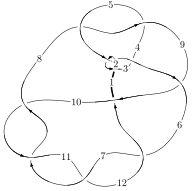
\includegraphics[width=112pt]{../../../GIT/diagram.site/Diagrams/png/2135_12n_0046.png}\\
\ \ \ A knot diagram\footnotemark}&
\allowdisplaybreaks
\textbf{Linearized knot diagam} \\
\cline{2-2}
 &
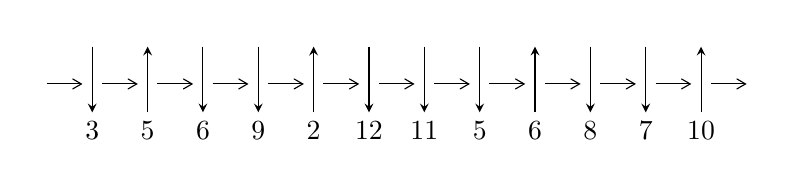
\begin{tikzpicture}[x=20pt, y=17pt]
	% nodes
	\node (C0) at (0, 0) {};
	\node (C1) at (1, 0) {};
	\node (C1U) at (1, +1) {};
	\node (C1D) at (1, -1) {3};

	\node (C2) at (2, 0) {};
	\node (C2U) at (2, +1) {};
	\node (C2D) at (2, -1) {5};

	\node (C3) at (3, 0) {};
	\node (C3U) at (3, +1) {};
	\node (C3D) at (3, -1) {6};

	\node (C4) at (4, 0) {};
	\node (C4U) at (4, +1) {};
	\node (C4D) at (4, -1) {9};

	\node (C5) at (5, 0) {};
	\node (C5U) at (5, +1) {};
	\node (C5D) at (5, -1) {2};

	\node (C6) at (6, 0) {};
	\node (C6U) at (6, +1) {};
	\node (C6D) at (6, -1) {12};

	\node (C7) at (7, 0) {};
	\node (C7U) at (7, +1) {};
	\node (C7D) at (7, -1) {11};

	\node (C8) at (8, 0) {};
	\node (C8U) at (8, +1) {};
	\node (C8D) at (8, -1) {5};

	\node (C9) at (9, 0) {};
	\node (C9U) at (9, +1) {};
	\node (C9D) at (9, -1) {6};

	\node (C10) at (10, 0) {};
	\node (C10U) at (10, +1) {};
	\node (C10D) at (10, -1) {8};

	\node (C11) at (11, 0) {};
	\node (C11U) at (11, +1) {};
	\node (C11D) at (11, -1) {7};

	\node (C12) at (12, 0) {};
	\node (C12U) at (12, +1) {};
	\node (C12D) at (12, -1) {10};
	\node (C13) at (13, 0) {};

	% arrows
	\draw[->,>={angle 60}]
	(C0) edge (C1) (C1) edge (C2) (C2) edge (C3) (C3) edge (C4) (C4) edge (C5) (C5) edge (C6) (C6) edge (C7) (C7) edge (C8) (C8) edge (C9) (C9) edge (C10) (C10) edge (C11) (C11) edge (C12) (C12) edge (C13) ;	\draw[->,>=stealth]
	(C1U) edge (C1D) (C2D) edge (C2U) (C3U) edge (C3D) (C4U) edge (C4D) (C5D) edge (C5U) (C6U) edge (C6D) (C7U) edge (C7D) (C8U) edge (C8D) (C9D) edge (C9U) (C10U) edge (C10D) (C11U) edge (C11D) (C12D) edge (C12U) ;
	\end{tikzpicture} \\
\hhline{~~} \\& 
\textbf{Solving Sequence} \\ \cline{2-2} 
 &
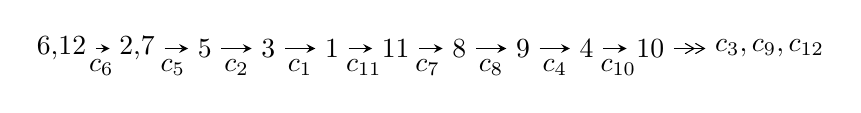
\begin{tikzpicture}[x=23pt, y=7pt]
	% node
	\node (A0) at (-1/8, 0) {6,12};
	\node (A1) at (17/16, 0) {2,7};
	\node (A2) at (17/8, 0) {5};
	\node (A3) at (25/8, 0) {3};
	\node (A4) at (33/8, 0) {1};
	\node (A5) at (41/8, 0) {11};
	\node (A6) at (49/8, 0) {8};
	\node (A7) at (57/8, 0) {9};
	\node (A8) at (65/8, 0) {4};
	\node (A9) at (73/8, 0) {10};
	\node (C1) at (1/2, -1) {$c_{6}$};
	\node (C2) at (13/8, -1) {$c_{5}$};
	\node (C3) at (21/8, -1) {$c_{2}$};
	\node (C4) at (29/8, -1) {$c_{1}$};
	\node (C5) at (37/8, -1) {$c_{11}$};
	\node (C6) at (45/8, -1) {$c_{7}$};
	\node (C7) at (53/8, -1) {$c_{8}$};
	\node (C8) at (61/8, -1) {$c_{4}$};
	\node (C9) at (69/8, -1) {$c_{10}$};
	\node (A10) at (11, 0) {$c_{3},c_{9},c_{12}$};

	% edge
	\draw[->,>=stealth]	
	(A0) edge (A1) (A1) edge (A2) (A2) edge (A3) (A3) edge (A4) (A4) edge (A5) (A5) edge (A6) (A6) edge (A7) (A7) edge (A8) (A8) edge (A9) ;
	\draw[->>,>={angle 60}]	
	(A9) edge (A10);
\end{tikzpicture} \\ 

\end{tabular} \\

\footnotetext{
The image of knot diagram is generated by the software ``\textbf{Draw programme}" developed by Andrew Bartholomew(\url{http://www.layer8.co.uk/maths/draw/index.htm\#Running-draw}), where we modified some parts for our purpose(\url{https://github.com/CATsTAILs/LinksPainter}).
}\phantom \\ \newline 
\centering \textbf{Ideals for irreducible components\footnotemark of $X_{\text{par}}$} 
 
\begin{align*}
I^u_{1}&=\langle 
- u^{27}-2 u^{26}+\cdots+2 b-6 u,\;u^{26}+2 u^{25}+\cdots+2 a+4,\;u^{28}+3 u^{27}+\cdots+6 u+1\rangle \\
I^u_{2}&=\langle 
- a u+b- u,\;u^3 a- u^2 a- u^3+a^2+3 a u-2 u,\;u^4- u^3+3 u^2-2 u+1\rangle \\
\\
\end{align*}
\raggedright * 2 irreducible components of $\dim_{\mathbb{C}}=0$, with total 36 representations.\\
\footnotetext{All coefficients of polynomials are rational numbers. But the coefficients are sometimes approximated in decimal forms when there is not enough margin.}
\newpage
\renewcommand{\arraystretch}{1}
\centering \section*{I. $I^u_{1}= \langle - u^{27}-2 u^{26}+\cdots+2 b-6 u,\;u^{26}+2 u^{25}+\cdots+2 a+4,\;u^{28}+3 u^{27}+\cdots+6 u+1 \rangle$}
\flushleft \textbf{(i) Arc colorings}\\
\begin{tabular}{m{7pt} m{180pt} m{7pt} m{180pt} }
\flushright $a_{6}=$&$\begin{pmatrix}1\\0\end{pmatrix}$ \\
\flushright $a_{12}=$&$\begin{pmatrix}0\\u\end{pmatrix}$ \\
\flushright $a_{2}=$&$\begin{pmatrix}-\frac{1}{2} u^{26}- u^{25}+\cdots-\frac{33}{2} u^2-2\\\frac{1}{2} u^{27}+u^{26}+\cdots+u^2+3 u\end{pmatrix}$ \\
\flushright $a_{7}=$&$\begin{pmatrix}1\\u^2\end{pmatrix}$ \\
\flushright $a_{5}=$&$\begin{pmatrix}-\frac{1}{2} u^{27}-\frac{3}{2} u^{26}+\cdots-15 u-2\\-\frac{1}{2} u^{27}- u^{26}+\cdots-3 u-1\end{pmatrix}$ \\
\flushright $a_{3}=$&$\begin{pmatrix}u^{27}+\frac{7}{2} u^{26}+\cdots+20 u+3\\-\frac{1}{2} u^{27}-2 u^{26}+\cdots-14 u^2-2 u\end{pmatrix}$ \\
\flushright $a_{1}=$&$\begin{pmatrix}u^7+4 u^5+4 u^3\\u^9+5 u^7+7 u^5+2 u^3+u\end{pmatrix}$ \\
\flushright $a_{11}=$&$\begin{pmatrix}u\\u^3+u\end{pmatrix}$ \\
\flushright $a_{8}=$&$\begin{pmatrix}u^2+1\\u^4+2 u^2\end{pmatrix}$ \\
\flushright $a_{9}=$&$\begin{pmatrix}- u^5-2 u^3+u\\u^5+3 u^3+u\end{pmatrix}$ \\
\flushright $a_{4}=$&$\begin{pmatrix}-\frac{3}{2} u^{27}-\frac{11}{2} u^{26}+\cdots-22 u-3\\\frac{1}{2} u^{27}+2 u^{26}+\cdots+14 u^2+2 u\end{pmatrix}$ \\
\flushright $a_{10}=$&$\begin{pmatrix}u^3+2 u\\u^5+3 u^3+u\end{pmatrix}$\\&\end{tabular}
\flushleft \textbf{(ii) Obstruction class $= -1$}\\~\\
\flushleft \textbf{(iii) Cusp Shapes $= \frac{5}{2} u^{27}+5 u^{26}+\cdots+21 u+\frac{1}{2}$}\\~\\
\newpage\renewcommand{\arraystretch}{1}
\flushleft \textbf{(iv) u-Polynomials at the component}\newline \\
\begin{tabular}{m{50pt}|m{274pt}}
Crossings & \hspace{64pt}u-Polynomials at each crossing \\
\hline $$\begin{aligned}c_{1}\end{aligned}$$&$\begin{aligned}
&u^{28}+5 u^{27}+\cdots+14 u+1
\end{aligned}$\\
\hline $$\begin{aligned}c_{2},c_{5}\end{aligned}$$&$\begin{aligned}
&u^{28}+5 u^{27}+\cdots+4 u+1
\end{aligned}$\\
\hline $$\begin{aligned}c_{3}\end{aligned}$$&$\begin{aligned}
&u^{28}-5 u^{27}+\cdots+5562 u+1321
\end{aligned}$\\
\hline $$\begin{aligned}c_{4},c_{8}\end{aligned}$$&$\begin{aligned}
&u^{28}+u^{27}+\cdots+384 u+256
\end{aligned}$\\
\hline $$\begin{aligned}c_{6},c_{7},c_{10}\\c_{11}\end{aligned}$$&$\begin{aligned}
&u^{28}-3 u^{27}+\cdots-6 u+1
\end{aligned}$\\
\hline $$\begin{aligned}c_{9}\end{aligned}$$&$\begin{aligned}
&u^{28}-3 u^{27}+\cdots-2 u+1
\end{aligned}$\\
\hline $$\begin{aligned}c_{12}\end{aligned}$$&$\begin{aligned}
&u^{28}+11 u^{27}+\cdots+184 u+209
\end{aligned}$\\
\hline
\end{tabular}\\~\\
\newpage\renewcommand{\arraystretch}{1}
\flushleft \textbf{(v) Riley Polynomials at the component}\newline \\
\begin{tabular}{m{50pt}|m{274pt}}
Crossings & \hspace{64pt}Riley Polynomials at each crossing \\
\hline $$\begin{aligned}c_{1}\end{aligned}$$&$\begin{aligned}
&y^{28}+41 y^{27}+\cdots+14 y+1
\end{aligned}$\\
\hline $$\begin{aligned}c_{2},c_{5}\end{aligned}$$&$\begin{aligned}
&y^{28}+5 y^{27}+\cdots+14 y+1
\end{aligned}$\\
\hline $$\begin{aligned}c_{3}\end{aligned}$$&$\begin{aligned}
&y^{28}+77 y^{27}+\cdots+102223598 y+1745041
\end{aligned}$\\
\hline $$\begin{aligned}c_{4},c_{8}\end{aligned}$$&$\begin{aligned}
&y^{28}+45 y^{27}+\cdots+344064 y+65536
\end{aligned}$\\
\hline $$\begin{aligned}c_{6},c_{7},c_{10}\\c_{11}\end{aligned}$$&$\begin{aligned}
&y^{28}+35 y^{27}+\cdots+6 y+1
\end{aligned}$\\
\hline $$\begin{aligned}c_{9}\end{aligned}$$&$\begin{aligned}
&y^{28}-49 y^{27}+\cdots+6 y+1
\end{aligned}$\\
\hline $$\begin{aligned}c_{12}\end{aligned}$$&$\begin{aligned}
&y^{28}-29 y^{27}+\cdots+2808126 y+43681
\end{aligned}$\\
\hline
\end{tabular}\\~\\
\newpage\flushleft \textbf{(vi) Complex Volumes and Cusp Shapes}
$$\begin{array}{c|c|c}  
\text{Solutions to }I^u_{1}& \I (\text{vol} + \sqrt{-1}CS) & \text{Cusp shape}\\
 \hline 
\begin{aligned}
u &= -0.546864 + 0.864620 I \\
a &= -1.78266 + 0.81365 I \\
b &= \phantom{-}0.938673 + 1.030660 I\end{aligned}
 & \phantom{-}12.0428 + 7.8502 I & \phantom{-}0.54802 - 5.73315 I \\ \hline\begin{aligned}
u &= -0.546864 - 0.864620 I \\
a &= -1.78266 - 0.81365 I \\
b &= \phantom{-}0.938673 - 1.030660 I\end{aligned}
 & \phantom{-}12.0428 - 7.8502 I & \phantom{-}0.54802 + 5.73315 I \\ \hline\begin{aligned}
u &= -0.512075 + 0.914815 I \\
a &= -0.310810 + 0.834490 I \\
b &= \phantom{-}1.006070 - 0.921537 I\end{aligned}
 & \phantom{-}12.40950 + 0.72573 I & \phantom{-}1.20101 - 1.26627 I \\ \hline\begin{aligned}
u &= -0.512075 - 0.914815 I \\
a &= -0.310810 - 0.834490 I \\
b &= \phantom{-}1.006070 + 0.921537 I\end{aligned}
 & \phantom{-}12.40950 - 0.72573 I & \phantom{-}1.20101 + 1.26627 I \\ \hline\begin{aligned}
u &= \phantom{-}0.041750 + 0.816332 I \\
a &= \phantom{-}0.984967 - 0.816170 I \\
b &= -0.730216 + 0.546904 I\end{aligned}
 & \phantom{-}2.67787 - 1.51352 I & \phantom{-}3.15826 + 2.96332 I \\ \hline\begin{aligned}
u &= \phantom{-}0.041750 - 0.816332 I \\
a &= \phantom{-}0.984967 + 0.816170 I \\
b &= -0.730216 - 0.546904 I\end{aligned}
 & \phantom{-}2.67787 + 1.51352 I & \phantom{-}3.15826 - 2.96332 I \\ \hline\begin{aligned}
u &= -0.755205 + 0.031373 I \\
a &= -0.154324 - 0.783184 I \\
b &= \phantom{-}0.955403 - 0.970517 I\end{aligned}
 & \phantom{-}9.53090 - 3.51075 I & -2.36490 + 2.10810 I \\ \hline\begin{aligned}
u &= -0.755205 - 0.031373 I \\
a &= -0.154324 + 0.783184 I \\
b &= \phantom{-}0.955403 + 0.970517 I\end{aligned}
 & \phantom{-}9.53090 + 3.51075 I & -2.36490 - 2.10810 I \\ \hline\begin{aligned}
u &= \phantom{-}0.429610 + 0.590805 I \\
a &= -1.30185 - 0.60397 I \\
b &= \phantom{-}0.291696 - 0.394438 I\end{aligned}
 & -0.15101 - 2.02920 I & -3.29658 + 3.20774 I \\ \hline\begin{aligned}
u &= \phantom{-}0.429610 - 0.590805 I \\
a &= -1.30185 + 0.60397 I \\
b &= \phantom{-}0.291696 + 0.394438 I\end{aligned}
 & -0.15101 + 2.02920 I & -3.29658 - 3.20774 I\\
 \hline 
 \end{array}$$\newpage$$\begin{array}{c|c|c}  
\text{Solutions to }I^u_{1}& \I (\text{vol} + \sqrt{-1}CS) & \text{Cusp shape}\\
 \hline 
\begin{aligned}
u &= -0.179883 + 0.692364 I \\
a &= \phantom{-}2.11541 - 0.80616 I \\
b &= -0.514946 - 1.029420 I\end{aligned}
 & \phantom{-}1.04465 + 3.25872 I & \phantom{-}1.94579 - 3.88394 I \\ \hline\begin{aligned}
u &= -0.179883 - 0.692364 I \\
a &= \phantom{-}2.11541 + 0.80616 I \\
b &= -0.514946 + 1.029420 I\end{aligned}
 & \phantom{-}1.04465 - 3.25872 I & \phantom{-}1.94579 + 3.88394 I \\ \hline\begin{aligned}
u &= \phantom{-}0.398241 + 0.347741 I \\
a &= -0.595350 + 0.678601 I \\
b &= -0.007486 + 0.515758 I\end{aligned}
 & -0.844911 - 0.963937 I & -7.23227 + 5.09608 I \\ \hline\begin{aligned}
u &= \phantom{-}0.398241 - 0.347741 I \\
a &= -0.595350 - 0.678601 I \\
b &= -0.007486 - 0.515758 I\end{aligned}
 & -0.844911 + 0.963937 I & -7.23227 - 5.09608 I \\ \hline\begin{aligned}
u &= \phantom{-}0.05307 + 1.53702 I \\
a &= -0.565559 + 0.333640 I \\
b &= \phantom{-}0.007766 + 0.841204 I\end{aligned}
 & \phantom{-}5.52882 - 2.13387 I & -4.00000 + 3.29212 I \\ \hline\begin{aligned}
u &= \phantom{-}0.05307 - 1.53702 I \\
a &= -0.565559 - 0.333640 I \\
b &= \phantom{-}0.007766 - 0.841204 I\end{aligned}
 & \phantom{-}5.52882 + 2.13387 I & -4.00000 - 3.29212 I \\ \hline\begin{aligned}
u &= \phantom{-}0.12702 + 1.57248 I \\
a &= -1.339830 - 0.272553 I \\
b &= \phantom{-}0.478138 - 0.445759 I\end{aligned}
 & \phantom{-}7.19200 - 4.05999 I & \phantom{-0.000000 } 0 \\ \hline\begin{aligned}
u &= \phantom{-}0.12702 - 1.57248 I \\
a &= -1.339830 + 0.272553 I \\
b &= \phantom{-}0.478138 + 0.445759 I\end{aligned}
 & \phantom{-}7.19200 + 4.05999 I & \phantom{-0.000000 } 0 \\ \hline\begin{aligned}
u &= -0.04195 + 1.63425 I \\
a &= \phantom{-}1.62168 + 0.08443 I \\
b &= -0.578450 - 1.150140 I\end{aligned}
 & \phantom{-}9.22292 + 4.03870 I & \phantom{-0.000000 } 0. - 2.65080 I \\ \hline\begin{aligned}
u &= -0.04195 - 1.63425 I \\
a &= \phantom{-}1.62168 - 0.08443 I \\
b &= -0.578450 + 1.150140 I\end{aligned}
 & \phantom{-}9.22292 - 4.03870 I & \phantom{-0.000000 -}0. + 2.65080 I\\
 \hline 
 \end{array}$$\newpage$$\begin{array}{c|c|c}  
\text{Solutions to }I^u_{1}& \I (\text{vol} + \sqrt{-1}CS) & \text{Cusp shape}\\
 \hline 
\begin{aligned}
u &= \phantom{-}0.01177 + 1.65893 I \\
a &= \phantom{-}1.41681 - 0.67494 I \\
b &= -0.955702 + 0.548085 I\end{aligned}
 & \phantom{-}11.38100 - 1.72426 I & \phantom{-}3.45594 + 0. I\phantom{ +0.000000I} \\ \hline\begin{aligned}
u &= \phantom{-}0.01177 - 1.65893 I \\
a &= \phantom{-}1.41681 + 0.67494 I \\
b &= -0.955702 - 0.548085 I\end{aligned}
 & \phantom{-}11.38100 + 1.72426 I & \phantom{-}3.45594 + 0. I\phantom{ +0.000000I} \\ \hline\begin{aligned}
u &= -0.16140 + 1.66866 I \\
a &= -1.98113 + 0.05979 I \\
b &= \phantom{-}0.93469 + 1.08649 I\end{aligned}
 & -18.7492 + 10.6138 I & \phantom{-0.000000 } 0. - 4.77955 I \\ \hline\begin{aligned}
u &= -0.16140 - 1.66866 I \\
a &= -1.98113 - 0.05979 I \\
b &= \phantom{-}0.93469 - 1.08649 I\end{aligned}
 & -18.7492 - 10.6138 I & \phantom{-0.000000 -}0. + 4.77955 I \\ \hline\begin{aligned}
u &= -0.14287 + 1.68669 I \\
a &= -1.04698 + 1.01839 I \\
b &= \phantom{-}1.072160 - 0.890015 I\end{aligned}
 & -18.0712 + 3.2992 I & \phantom{-0.000000 } 0 \\ \hline\begin{aligned}
u &= -0.14287 - 1.68669 I \\
a &= -1.04698 - 1.01839 I \\
b &= \phantom{-}1.072160 + 0.890015 I\end{aligned}
 & -18.0712 - 3.2992 I & \phantom{-0.000000 } 0 \\ \hline\begin{aligned}
u &= -0.221218 + 0.191391 I \\
a &= -2.06037 + 1.41739 I \\
b &= -0.397798 + 0.843645 I\end{aligned}
 & -0.31537 - 1.65529 I & -2.65586 + 5.38450 I \\ \hline\begin{aligned}
u &= -0.221218 - 0.191391 I \\
a &= -2.06037 - 1.41739 I \\
b &= -0.397798 - 0.843645 I\end{aligned}
 & -0.31537 + 1.65529 I & -2.65586 - 5.38450 I\\
 \hline 
 \end{array}$$\newpage\newpage\renewcommand{\arraystretch}{1}
\centering \section*{II. $I^u_{2}= \langle - a u+b- u,\;u^3 a- u^2 a- u^3+a^2+3 a u-2 u,\;u^4- u^3+3 u^2-2 u+1 \rangle$}
\flushleft \textbf{(i) Arc colorings}\\
\begin{tabular}{m{7pt} m{180pt} m{7pt} m{180pt} }
\flushright $a_{6}=$&$\begin{pmatrix}1\\0\end{pmatrix}$ \\
\flushright $a_{12}=$&$\begin{pmatrix}0\\u\end{pmatrix}$ \\
\flushright $a_{2}=$&$\begin{pmatrix}a\\a u+u\end{pmatrix}$ \\
\flushright $a_{7}=$&$\begin{pmatrix}1\\u^2\end{pmatrix}$ \\
\flushright $a_{5}=$&$\begin{pmatrix}u^3- a u- u^2+a+2 u\\a u+u-1\end{pmatrix}$ \\
\flushright $a_{3}=$&$\begin{pmatrix}u^3- u^2+a+3 u-1\\a u+u-1\end{pmatrix}$ \\
\flushright $a_{1}=$&$\begin{pmatrix}-1\\0\end{pmatrix}$ \\
\flushright $a_{11}=$&$\begin{pmatrix}u\\u^3+u\end{pmatrix}$ \\
\flushright $a_{8}=$&$\begin{pmatrix}u^2+1\\u^3- u^2+2 u-1\end{pmatrix}$ \\
\flushright $a_{9}=$&$\begin{pmatrix}u^2+1\\u^3- u^2+2 u-1\end{pmatrix}$ \\
\flushright $a_{4}=$&$\begin{pmatrix}u^3- a u- u^2+a+2 u\\a u+u-1\end{pmatrix}$ \\
\flushright $a_{10}=$&$\begin{pmatrix}u^3+2 u\\u^3- u^2+2 u-1\end{pmatrix}$\\&\end{tabular}
\flushleft \textbf{(ii) Obstruction class $= 1$}\\~\\
\flushleft \textbf{(iii) Cusp Shapes $= - u^2 a+4 u^3-4 a u-5 u^2+a+9 u-5$}\\~\\
\newpage\renewcommand{\arraystretch}{1}
\flushleft \textbf{(iv) u-Polynomials at the component}\newline \\
\begin{tabular}{m{50pt}|m{274pt}}
Crossings & \hspace{64pt}u-Polynomials at each crossing \\
\hline $$\begin{aligned}c_{1},c_{3},c_{5}\end{aligned}$$&$\begin{aligned}
&(u^2- u+1)^4
\end{aligned}$\\
\hline $$\begin{aligned}c_{2}\end{aligned}$$&$\begin{aligned}
&(u^2+u+1)^4
\end{aligned}$\\
\hline $$\begin{aligned}c_{4},c_{8}\end{aligned}$$&$\begin{aligned}
&u^8
\end{aligned}$\\
\hline $$\begin{aligned}c_{6},c_{7}\end{aligned}$$&$\begin{aligned}
&(u^4- u^3+3 u^2-2 u+1)^2
\end{aligned}$\\
\hline $$\begin{aligned}c_{9},c_{12}\end{aligned}$$&$\begin{aligned}
&(u^4+u^3+u^2+1)^2
\end{aligned}$\\
\hline $$\begin{aligned}c_{10},c_{11}\end{aligned}$$&$\begin{aligned}
&(u^4+u^3+3 u^2+2 u+1)^2
\end{aligned}$\\
\hline
\end{tabular}\\~\\
\newpage\renewcommand{\arraystretch}{1}
\flushleft \textbf{(v) Riley Polynomials at the component}\newline \\
\begin{tabular}{m{50pt}|m{274pt}}
Crossings & \hspace{64pt}Riley Polynomials at each crossing \\
\hline $$\begin{aligned}c_{1},c_{2},c_{3}\\c_{5}\end{aligned}$$&$\begin{aligned}
&(y^2+y+1)^4
\end{aligned}$\\
\hline $$\begin{aligned}c_{4},c_{8}\end{aligned}$$&$\begin{aligned}
&y^8
\end{aligned}$\\
\hline $$\begin{aligned}c_{6},c_{7},c_{10}\\c_{11}\end{aligned}$$&$\begin{aligned}
&(y^4+5 y^3+7 y^2+2 y+1)^2
\end{aligned}$\\
\hline $$\begin{aligned}c_{9},c_{12}\end{aligned}$$&$\begin{aligned}
&(y^4+y^3+3 y^2+2 y+1)^2
\end{aligned}$\\
\hline
\end{tabular}\\~\\
\newpage\flushleft \textbf{(vi) Complex Volumes and Cusp Shapes}
$$\begin{array}{c|c|c}  
\text{Solutions to }I^u_{2}& \I (\text{vol} + \sqrt{-1}CS) & \text{Cusp shape}\\
 \hline 
\begin{aligned}
u &= \phantom{-}0.395123 + 0.506844 I \\
a &= \phantom{-}0.541116 + 0.214920 I \\
b &= \phantom{-}0.500000 + 0.866025 I\end{aligned}
 & -0.211005 + 0.614778 I & -1.64912 + 1.57080 I \\ \hline\begin{aligned}
u &= \phantom{-}0.395123 + 0.506844 I \\
a &= -1.58443 - 1.44211 I \\
b &= \phantom{-}0.500000 - 0.866025 I\end{aligned}
 & -0.21101 - 3.44499 I & -4.65255 + 7.52635 I \\ \hline\begin{aligned}
u &= \phantom{-}0.395123 - 0.506844 I \\
a &= \phantom{-}0.541116 - 0.214920 I \\
b &= \phantom{-}0.500000 - 0.866025 I\end{aligned}
 & -0.211005 - 0.614778 I & -1.64912 - 1.57080 I \\ \hline\begin{aligned}
u &= \phantom{-}0.395123 - 0.506844 I \\
a &= -1.58443 + 1.44211 I \\
b &= \phantom{-}0.500000 + 0.866025 I\end{aligned}
 & -0.21101 + 3.44499 I & -4.65255 - 7.52635 I \\ \hline\begin{aligned}
u &= \phantom{-}0.10488 + 1.55249 I \\
a &= -0.423047 - 0.283088 I \\
b &= \phantom{-}0.500000 + 0.866025 I\end{aligned}
 & \phantom{-}6.79074 - 1.13408 I & \phantom{-}1.80063 - 0.49697 I \\ \hline\begin{aligned}
u &= \phantom{-}0.10488 + 1.55249 I \\
a &= -1.53364 - 0.35811 I \\
b &= \phantom{-}0.500000 - 0.866025 I\end{aligned}
 & \phantom{-}6.79074 - 5.19385 I & -1.99896 + 6.53786 I \\ \hline\begin{aligned}
u &= \phantom{-}0.10488 - 1.55249 I \\
a &= -0.423047 + 0.283088 I \\
b &= \phantom{-}0.500000 - 0.866025 I\end{aligned}
 & \phantom{-}6.79074 + 1.13408 I & \phantom{-}1.80063 + 0.49697 I \\ \hline\begin{aligned}
u &= \phantom{-}0.10488 - 1.55249 I \\
a &= -1.53364 + 0.35811 I \\
b &= \phantom{-}0.500000 + 0.866025 I\end{aligned}
 & \phantom{-}6.79074 + 5.19385 I & -1.99896 - 6.53786 I\\
 \hline 
 \end{array}$$\newpage
\newpage\renewcommand{\arraystretch}{1}
\centering \section*{ III. u-Polynomials}
\begin{tabular}{m{50pt}|m{274pt}}
Crossings & \hspace{64pt}u-Polynomials at each crossing \\
\hline $$\begin{aligned}c_{1}\end{aligned}$$&$\begin{aligned}
&((u^2- u+1)^4)(u^{28}+5 u^{27}+\cdots+14 u+1)
\end{aligned}$\\
\hline $$\begin{aligned}c_{2}\end{aligned}$$&$\begin{aligned}
&((u^2+u+1)^4)(u^{28}+5 u^{27}+\cdots+4 u+1)
\end{aligned}$\\
\hline $$\begin{aligned}c_{3}\end{aligned}$$&$\begin{aligned}
&((u^2- u+1)^4)(u^{28}-5 u^{27}+\cdots+5562 u+1321)
\end{aligned}$\\
\hline $$\begin{aligned}c_{4},c_{8}\end{aligned}$$&$\begin{aligned}
&u^8(u^{28}+u^{27}+\cdots+384 u+256)
\end{aligned}$\\
\hline $$\begin{aligned}c_{5}\end{aligned}$$&$\begin{aligned}
&((u^2- u+1)^4)(u^{28}+5 u^{27}+\cdots+4 u+1)
\end{aligned}$\\
\hline $$\begin{aligned}c_{6},c_{7}\end{aligned}$$&$\begin{aligned}
&((u^4- u^3+3 u^2-2 u+1)^2)(u^{28}-3 u^{27}+\cdots-6 u+1)
\end{aligned}$\\
\hline $$\begin{aligned}c_{9}\end{aligned}$$&$\begin{aligned}
&((u^4+u^3+u^2+1)^2)(u^{28}-3 u^{27}+\cdots-2 u+1)
\end{aligned}$\\
\hline $$\begin{aligned}c_{10},c_{11}\end{aligned}$$&$\begin{aligned}
&((u^4+u^3+3 u^2+2 u+1)^2)(u^{28}-3 u^{27}+\cdots-6 u+1)
\end{aligned}$\\
\hline $$\begin{aligned}c_{12}\end{aligned}$$&$\begin{aligned}
&((u^4+u^3+u^2+1)^2)(u^{28}+11 u^{27}+\cdots+184 u+209)
\end{aligned}$\\
\hline
\end{tabular}\newpage\renewcommand{\arraystretch}{1}
\centering \section*{ IV. Riley Polynomials}
\begin{tabular}{m{50pt}|m{274pt}}
Crossings & \hspace{64pt}Riley Polynomials at each crossing \\
\hline $$\begin{aligned}c_{1}\end{aligned}$$&$\begin{aligned}
&((y^2+y+1)^4)(y^{28}+41 y^{27}+\cdots+14 y+1)
\end{aligned}$\\
\hline $$\begin{aligned}c_{2},c_{5}\end{aligned}$$&$\begin{aligned}
&((y^2+y+1)^4)(y^{28}+5 y^{27}+\cdots+14 y+1)
\end{aligned}$\\
\hline $$\begin{aligned}c_{3}\end{aligned}$$&$\begin{aligned}
&((y^2+y+1)^4)(y^{28}+77 y^{27}+\cdots+1.02224\times10^{8} y+1745041)
\end{aligned}$\\
\hline $$\begin{aligned}c_{4},c_{8}\end{aligned}$$&$\begin{aligned}
&y^8(y^{28}+45 y^{27}+\cdots+344064 y+65536)
\end{aligned}$\\
\hline $$\begin{aligned}c_{6},c_{7},c_{10}\\c_{11}\end{aligned}$$&$\begin{aligned}
&((y^4+5 y^3+7 y^2+2 y+1)^2)(y^{28}+35 y^{27}+\cdots+6 y+1)
\end{aligned}$\\
\hline $$\begin{aligned}c_{9}\end{aligned}$$&$\begin{aligned}
&((y^4+y^3+3 y^2+2 y+1)^2)(y^{28}-49 y^{27}+\cdots+6 y+1)
\end{aligned}$\\
\hline $$\begin{aligned}c_{12}\end{aligned}$$&$\begin{aligned}
&((y^4+y^3+3 y^2+2 y+1)^2)(y^{28}-29 y^{27}+\cdots+2808126 y+43681)
\end{aligned}$\\
\hline
\end{tabular}
\vskip 2pc
\end{document}